\section{Модель}\subsection{СК и ОК}
\begin{frame}{Модели системы и объекта контроля}{Предметная область}
    \begin{minipage}[t]{0.57\linewidth}
        \textbf{\tiny Рабочее место}
        \center{\includegraphics<1->[width=1\linewidth,keepaspectratio]{scheme_presentation}}
    \end{minipage}
    \hfill
    \begin{minipage}[t]{0.4\linewidth}
        \begin{itemize}
            \item[АНПА] автономный необитаемый подводный аппарат
            \item[АРМ] автоматизированное рабочее место
            \item[БГР] блок гальванической развязки
            \item[ОК]  объект контроля
            \item[ПЛК] программируемый логический контроллер
            \item[СК]  система контроля            
        \end{itemize}
    \end{minipage}\pause
    \vspace{3pt}
    \centering{\fbox{\parbox{.8\textwidth}{АНПА предназначен для поиска скоплений \textit{планктона},
                \textit{рыбных косяков} или \textit{китов} путем анализа испущенной специализированной зондирующей посылки.}}}
    % \centering{\leadingOrganizationTitle}
\end{frame}





\subsection{Общесистемные сущности модели}
\begin{frame}{Общесистемные сущности модели АНПА}{Объекты --- Функции --- Действия. Имитируемые сигналы}
    \vspace{-5mm}{\tiny\begin{equation*}\begin{split}
        C_1 = &A \times B,\qquad
        C_2 = \begin{pmatrix} \sum_{j=1}^l c_{1\,1j} \\ \ldots \\ \sum_{j=1}^l c_{1\,mj} \end{pmatrix},\qquad
        C_3 = \frac{C_2}{l},{}\\
        \left. C_3^* \right|_{l \equiv 6} = &
                 \left( 0.67\;\; 0.67\;\; \textcolor{\thirdcolor}{1.33}\;\; 0.67\;\; \textcolor{\thirdcolor}{1.33}\;\; 0.67\;\; 0.83\;\; 0.83\;\; 
                        0.33\;\; \textcolor{\secondcolor}{1.5}\;\;\textcolor{\secondcolor}{1.5}\;\; 0.67\;\; \textcolor{\firstcolor}{2.00}\;\; 0.67 \right)^T\,.
    \end{split}\end{equation*}}
    \textbf{Общесистемные сущности при $K_{min} = \overline{C_3^*} = 0.98$}:
    \begin{itemize}
        \item<first@1->[2.0]  блок управления батареей;
        \item<second@1->[1.5] рулевые машинки, рулевой привод;
        \item<third@1->[1.33] анализатор приемо-излучательного тракта СПО и установщик~курса.
    \end{itemize}
    %
    \hrule{}\begin{enumerate}
        \item<2-> Внешние
        \begin{itemize}
            \item<2->[Глубина] $h = \{h_1, h_2, \ldots\, h_n\} = \{F(\vec p(t); t_1), F(\vec p(t); t_2), \ldots, F(\vec p(t); t_n)\}$;
            \item<3->[Эхо-сигнал] $s_j \Rightarrow \{r_j\} \cup \{e_j\} \ne \emptyset:\,\{r_j\} \cap \{e_j\} = \emptyset$,
                где $\{e_j\}$ -- авария.
        \end{itemize}\vspace{5pt}
        \item<2-> Внутренние
        \begin{itemize}
            \item<4->[Напряжения] $U_i = \{U_1, U_2, \ldots, U_j\};\quad U_i \in [U_i^{min}, U_i^{max}]$,
            \item<4->[Токи] $I_\Sigma = \sum_k^N I_k + \hat I;\quad I_k \in [I_k^{min}, I_k^{max}];\quad \hat I \in [\hat I^{min}, \hat I^{max}]$;
            \item<5->[СУД] $\langle f; Q \rangle$ вращения вала \textit{двигателя} в виде ШИМ сигнала;
            \item<6->[Руление] $\langle s_j, \{r_j\} \rangle \Rightarrow \omega_i = \omega_i(s_j, \{r_j\})$.
        \end{itemize}    
    \end{enumerate}
\end{frame}






\section{Онтология}
\begin{frame}{Онтология модели АНПА}{\protege}
    \begin{center}

        {\huge Онтология} --- это способ показать свойства предметной области и то, как они связаны,
            определив набор понятий и категорий, которые представляют предмет.
    \end{center}
\end{frame}






\section{Реализация}\subsection{Таксономия классов}
\begin{frame}{Таксономия классов}
    \vspace{-1mm}\hspace{-5mm}\begin{minipage}[c]{0.4\linewidth}
        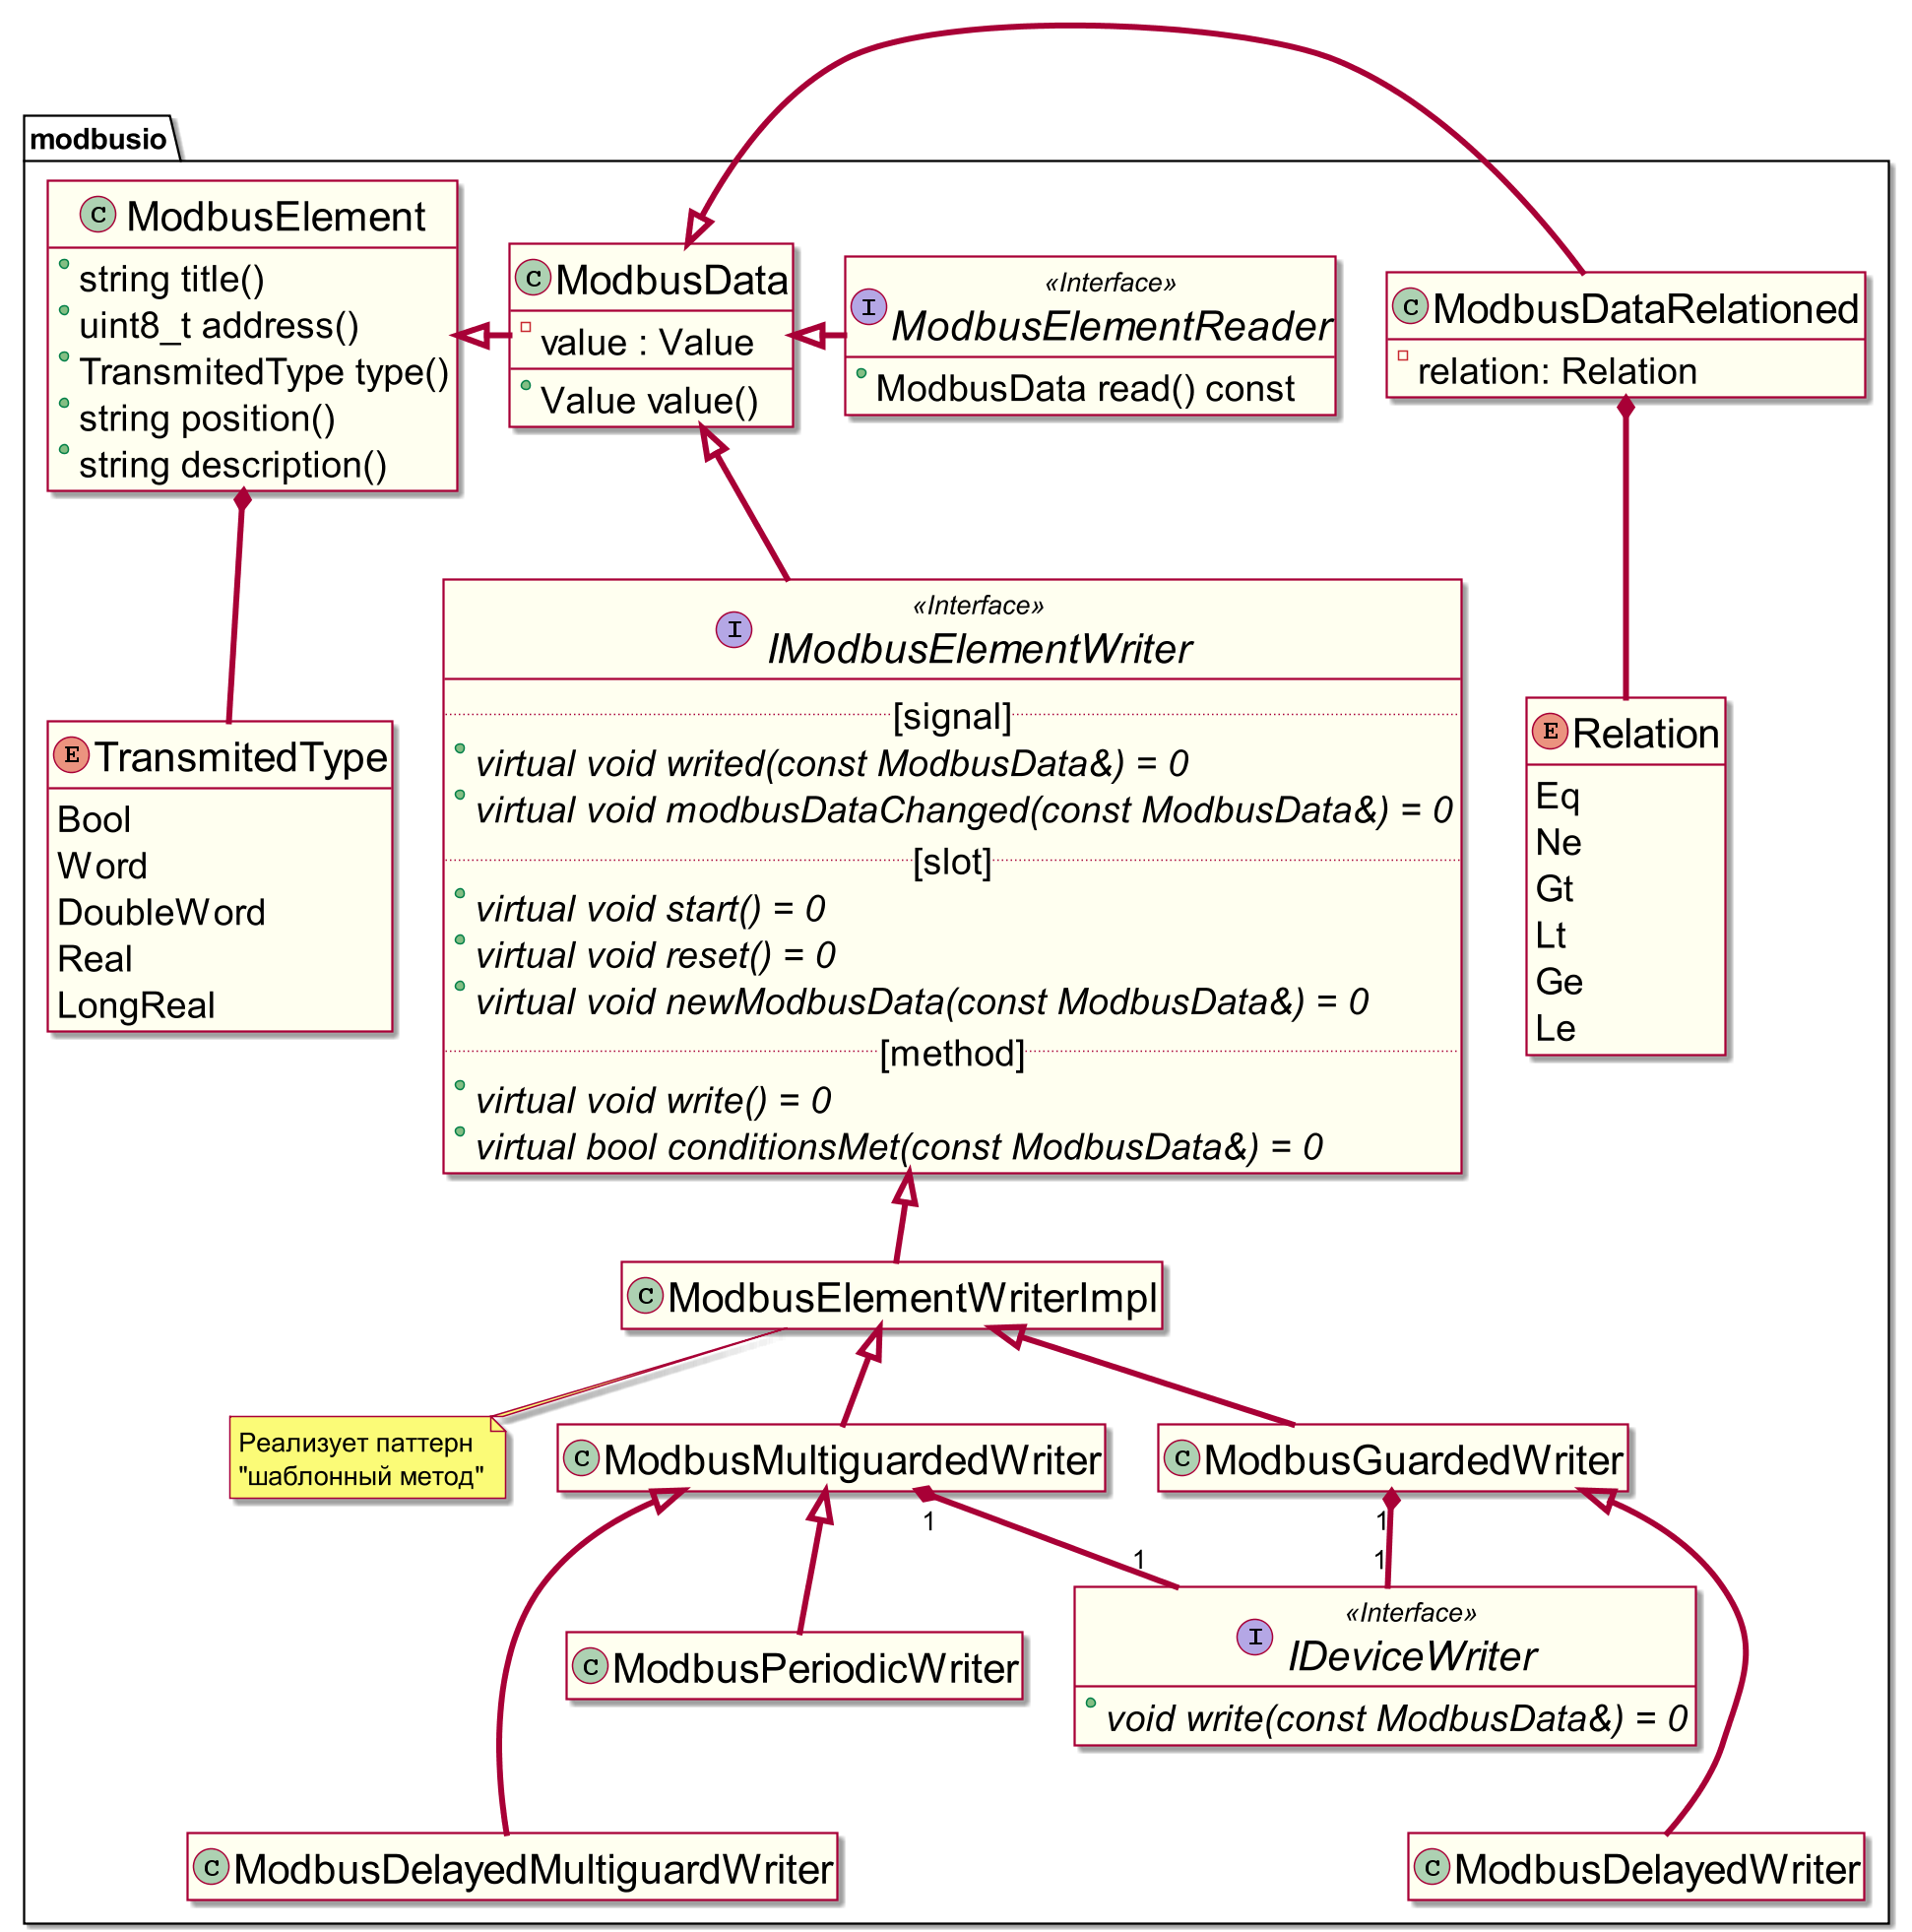
\includegraphics[height=.8\textheight]{modbus_class_relationship_short.png}
    \end{minipage}
    %
    \hspace{25mm}\begin{minipage}[c]{0.4\linewidth}
    {\tiny\begin{enumerate}
        \item \texttt{ModbusElement}, \texttt{TransmitedType}
        \item \texttt{ModbusData}, \texttt{ModbusDataRelationed} \eqref{eq:relation}
        \item Интерфейс~\texttt{IModbusElementWriter}
        \begin{itemize}
            \item {\tiny сигналы о записи и изменении}
            \item {\tiny слоты на запуск, останов и обработку новых данных}
            \item {\tiny проверка условий, запись}
        \end{itemize}
        \item Реализации интерфейса
        \item Делегирование интерфейсу \texttt{IDeviceWriter}
    \end{enumerate}}
\end{minipage}
    \begin{equation}\label{eq:relation}
        \mathcal{A} \left(\mathcal{M}_i;\, r \right) = a \in \{0, 1\}\,, \qquad
        r \in \{\equiv,\ne,>,<,\ge,\le\}
    \end{equation}
\end{frame}





\subsection{Алгоритм работы имитатора}
\begin{frame}{Алгоритм работы имитатора}
    \begin{center}
        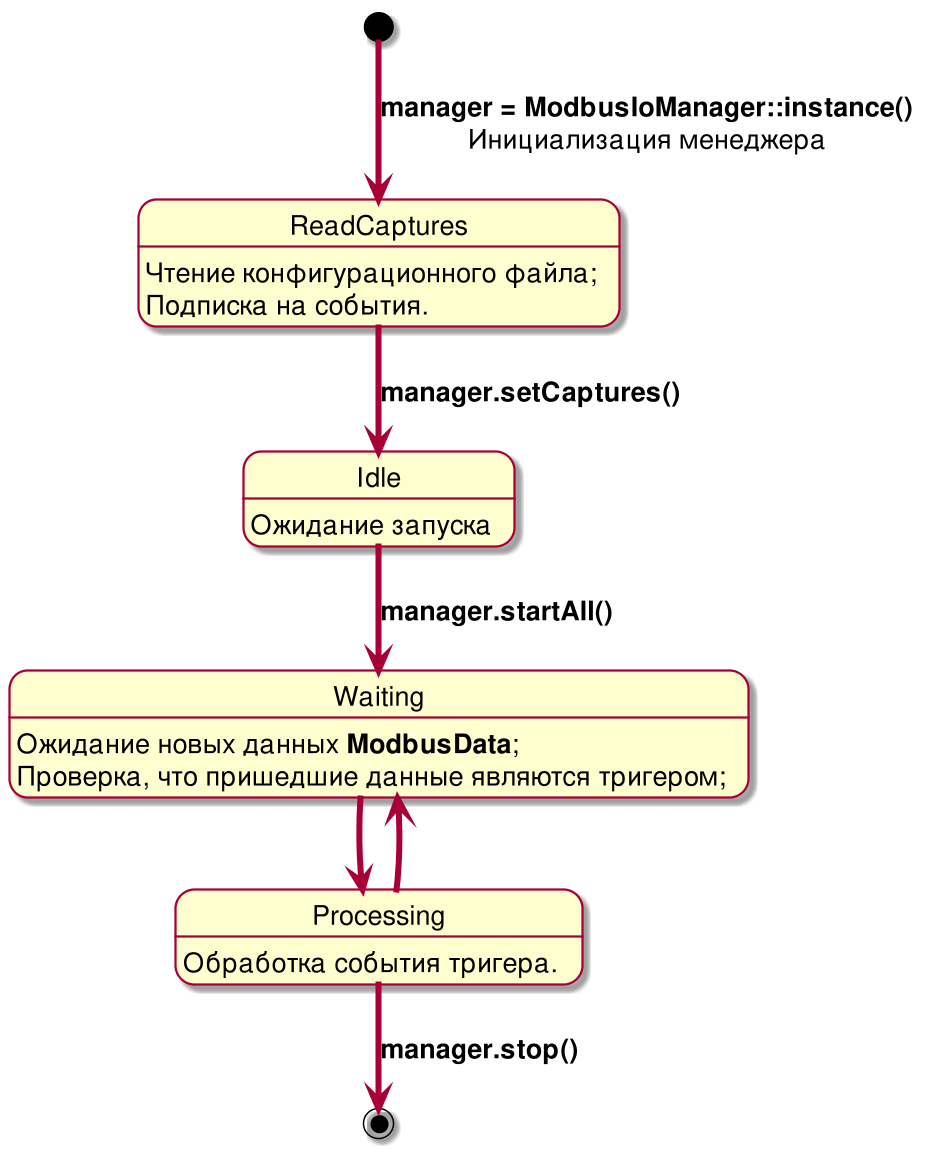
\includegraphics[height=.8\textheight]{modbusiomanager_state_diagram.png}
    \end{center}
\end{frame}






\subsection{Сценарий}
\begin{frame}{Формирование сценария}
    \textbf{Настройка:}
    \begin{enumerate}
        \item Конфигурация описывается в \texttt{XML} файле.
        \item Используется схема разметки \texttt{XSD}.
    \end{enumerate}
    \textbf{Сценарий содержит:}
    \begin{enumerate}
        \item Значения по умолчанию.
        \item Правила изменения состояния.
    \end{enumerate}
\end{frame}